  \documentclass[11pt,a4paper]{article}
  \usepackage[utf8]{inputenc}
  \usepackage{amsmath}
  \usepackage{amsfonts}
  \usepackage{graphicx}
  \usepackage[table,xcdraw]{xcolor}
  \usepackage{gensymb} %para el simbolo de los grados celsius


  \DeclareUnicodeCharacter{00A0}{ } %este rollo es para evitar un error por la aparición de un caracter invisible e hijo de puta

  \usepackage{caption}
  \usepackage{subcaption}

  \renewcommand{\familydefault}{\sfdefault} % cambiamos la fuente a una sans

  \usepackage{float} % para que floten las imagenes o algo asi...
  \usepackage{wallpaper} %paquete para usar una imagen como encabezado!
  \usepackage{hyperref} %para usar hypervinculos 
  \usepackage[export]{adjustbox} %para usar marcos en imagenes
  \usepackage{eurosym} % para el euro
  \usepackage{transparent} %para las marcas de agua
  \usepackage{eso-pic}  %para las marcas de agua

  \definecolor{azul_marcos}{RGB}{0,128,159} %defino el color azul de los marcos
  \usepackage{sectsty} %esto es para cambiar el color de las fuentes creo
  \renewcommand{\familydefault}{\sfdefault} % cambiamos la fuente a una sans
  \sectionfont{\color{azul_marcos}}  % sets colour of sections
  \subsectionfont{\color{azul_marcos}}  % sets colour of sections


  \usepackage{pdfpages} %para insertar pdfs
  \usepackage{amssymb}
  \usepackage{pstcol} % para color
  \usepackage{pst-node} % para diagramas
  \usepackage{pst-plot} % para representacion de dat
  \usepackage[spanish]{babel}
  \addto\captionsspanish{\renewcommand\chaptername{Bloque}}
  %\usepackage[total={18cm,21cm},top=2cm, left=2cm]{geometry}
  \usepackage{anysize}
  \pagestyle{plain}
  %\markboth{left head}{right head}
  %\markright{Guía de impresión PETG Tech}
  \marginsize{3cm}{2cm}{2.5cm}{1cm}
  \title{Guía de impresión PETG Tech}
  \date{}

  %configuracion de la marca de agua
  \AddToShipoutPicture{
      \put(0,0){
          \parbox[b][\paperheight]{\paperwidth}{%
              \vfill
              \centering
              {\transparent{0.1}
\includegraphics[scale=1.25]{FOTOS/logofff}}%
              \vfill
          }
      }
  }

  \begin{document}
  \ULCornerWallPaper{1}{FOTOS/header}
  \LLCornerWallPaper{1}{FOTOS/footer}
  %\maketitle
  %\tableofcontents
  
\includepdf{PDF/PORTADA.pdf}
  \section{Qu’est-ce qu’un filament PETG Tech?}PETG Tech est un filament pour impression 3D FFF / FDM du polyéthylène téréphtalate glycol (P.E.T.G.) conçu pour combiner le meilleur de PLA et ABS étant un résistant thermoplastique et facile à imprimer.
  \begin{figure}[H]
  \centering
  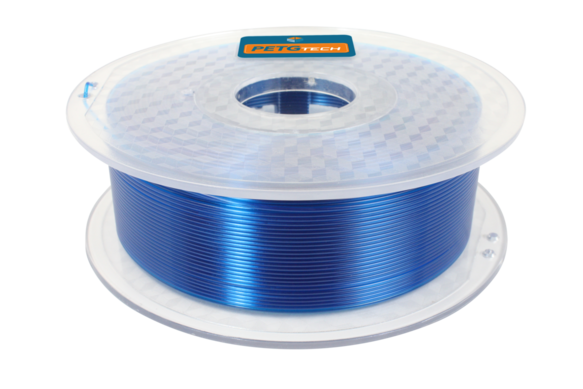
\includegraphics[width=0.5\textwidth,cfbox=azul_marcos 1pt 0pt]{FOTOS/PETGKILOAZUL}
  \end{figure}
  \section{Pourquoi devriez-vous utiliser le filament PETG Tech 3D?}
PETG Tech est l’un des filaments les plus polyvalents du marché puisqu’ il combine les meilleures propriétés d’autres matériaux.
  \begin{itemize}
  \item Le PETG est très résistant, presque autant que l'ABS, d’où son utilisation pour la construction des pièces qui risquent de  subir des contraintes mécaniques par traction, pression ou impact.
  \item Le PETG résiste également à la température mieux que le PLA et il a une bonne résistance aux produits chimiques et les solvants. Il résiste également à l’exposition aux UV mieux que le PLA et l’ABS.
  \item En plus, le filament de PETG présente beaucoup moins de « déformation » (ou tendance à se déformer lors du refroidissement) que l’ABS, et en suivant les bonnes méthodes, on peut le contrôler parfaitement. Alors, c’est pour cette raison que le filament PETG, et contrairement aux autres filament, permet l’impression de gros volumes dans les imprimantes à usage domestique.
  \item Etant un matériau moins hygroscopique il est plus facilement et aussi mieux préservé que le PLA.
  \item Bien que le filament PETG n’est pas certifié pour être en contact avec les aliments (sécurité alimentaire FDA)en revanche le bouletage à partir duquel il est fabriqué, est certifié , et cela le rend plus convenable au contact avec les aliments que d’autres matériaux. Plus tard, nous analyserons en profondeur cet aspect.
  \item Le PETG est naturellement translucide et brillant. Bien qu’il est aussi vendu en couleurs opaques, ces couleurs conservent une finition brillante.
  \item PETG est un matériau recyclable et biodégradable, à l’instar de PLA.
  \end{itemize}
  Voici un tableau comparatif entre le PETG l’APL et l’ABS:
  \begin{table}[H]
  \centering
  \begin{tabular}{l|c|c|c|}
  \cline{2-4}
                                                                                        & \cellcolor[HTML]{FFFFFF}PLA & \cellcolor[HTML]{FFFFFF}ABS & \cellcolor[HTML]{FFFFFF}PETG \\ \hline
  \rowcolor[HTML]{FFFFFF} 
  \multicolumn{1}{|l|}{\cellcolor[HTML]{FFFFFF}Résistant aux chocs élevés}          &                             & X                           & X                            \\ \hline
  \rowcolor[HTML]{FFFFFF} 
  \multicolumn{1}{|l|}{\cellcolor[HTML]{FFFFFF}Faible déformation (warping)} & X                           &                             & X                            \\ \hline
  \rowcolor[HTML]{FFFFFF} 
  \multicolumn{1}{|l|}{\cellcolor[HTML]{FFFFFF}Absorbe une faible humidité}                    &                             & X                           & X                            \\ \hline
  \rowcolor[HTML]{FFFFFF} 
  \multicolumn{1}{|l|}{\cellcolor[HTML]{FFFFFF}Biodégradable}                           & X                           &                             & X                            \\ \hline
  \rowcolor[HTML]{FFFFFF} 
  \multicolumn{1}{|l|}{\cellcolor[HTML]{FFFFFF}Sécurité alimentaire de la FDA *}                       &                             &                             & X                            \\ \hline
  \rowcolor[HTML]{FFFFFF} 
  \multicolumn{1}{|l|}{\cellcolor[HTML]{FFFFFF}Bonne résistance à la lumière UV}            &                             &                             & X                            \\ \hline
  \rowcolor[HTML]{FFFFFF} 
  \multicolumn{1}{|l|}{\cellcolor[HTML]{FFFFFF}Pas d'odeur lors de l'impression}                 & X                           &                             & X                            \\ \hline
  \end{tabular}
  \end{table}
  \section{Données techniques et paramètres d’impression}
  \begin{table}[H]
  \centering
  \caption*{Fiche technique}
  \begin{tabular}{|
  >{\columncolor[HTML]{FFFFFF}}l |
  >{\columncolor[HTML]{FFFFFF}}c |}
  \hline
  \multicolumn{1}{|c|}{\cellcolor[HTML]{FFFFFF}\textbf{Matière}}   & Tereftalato de polietileno glycol   \\ \hline
  \textbf{Couleurs disponibles}              & 5 (3 translucide, 2 opaque)                 \\ \hline
  \textbf{Formats disponibles}             & 1kg, 250gr         \\ \hline
  \textbf{Température de déformation à la chaleur} & 70               \\ \hline
  \textbf{Température de fusion}            & 200ºC              \\ \hline
  \textbf{Température de décomposition}    & \textgreater 280ºC \\ \hline
  \textbf{Densité}                         & 1.27 gr / cm3      \\ \hline
  \textbf{Résistance aux chocs}                         & 100 kg-cm / cm      \\ \hline
  \textbf{Étirement maximal}              & 140\%              \\ \hline
  \end{tabular}
  \end{table}

  %TABLA PARAMETROS IMPRESION MEDIA

  \begin{table}[H]
  \centering
  \caption*{Paramètres d’impression moyenne}
  \begin{tabular}{|
  >{\columncolor[HTML]{FFFFFF}}l |
  >{\columncolor[HTML]{FFFFFF}}c |}
  \hline
  \multicolumn{1}{|c|}{\cellcolor[HTML]{FFFFFF}\textbf{Température d'impression recommandé}} & 245º              \\ \hline
  \textbf{L'impression de vitesse recommandée}                         & 55 mm/s              \\ \hline
  \textbf{Hauteur couche optimale}                                  &  0.2 mm        \\ \hline
  \textbf{Température du lit chaud}                                  &  70º - 85º        \\ \hline
  \textbf{Ventilateur de couche}                                  &  75\%        \\ \hline
  \textbf{Extrusion multiplier **}                                  &  85\% / 100\%        \\ \hline

  \textbf{Rétraction ***}                                      & Normale ou augmentée                 \\ \hline
  \end{tabular}
  \end{table}

  %TABLA PARAMETROS RESISTENCIA

  \begin{table}[H]
  \centering
  \caption*{Paramètres d'impression recommandés pour une résistance maximale et moins de transparence *}
  \begin{tabular}{|
  >{\columncolor[HTML]{FFFFFF}}l |
  >{\columncolor[HTML]{FFFFFF}}c |}
  \hline
  \multicolumn{1}{|c|}{\cellcolor[HTML]{FFFFFF}\textbf{Température d'impression recommandé}} & 260º              \\ \hline
  \textbf{L'impression de vitesse recommandée}                         & 40 mm/s              \\ \hline
  \textbf{Hauteur couche optimale}                                  &  0.2 mm        \\ \hline
  \textbf{Température du lit chaud}                                  &  70º - 85º        \\ \hline
  \textbf{Ventilateur de couche}                                  &  Désactivé       \\ \hline
  \textbf{Extrusion multiplier **}                                  &  85\% / 100\%        \\ \hline

  \textbf{Rétraction ***}                                      & Normale ou augmentée                 \\ \hline
  \end{tabular}
  \end{table}

  %TABLA PARAMETROS TRANSPARENCIA

  \begin{table}[H]
  \centering
  \caption*{Paramètres d'impression recommandés pour une transparence maximale et moins de résistance **}
  \begin{tabular}{|
  >{\columncolor[HTML]{FFFFFF}}l |
  >{\columncolor[HTML]{FFFFFF}}c |}
\hline
\multicolumn{1}{|c|}{\cellcolor[HTML]{FFFFFF}\textbf{Température d'impression recommandé}} & 235º - 240º              \\ \hline
\textbf{L'impression de vitesse recommandée}                         & 70 mm/s              \\ \hline
\textbf{Hauteur couche optimale}                                  &  0.3 mm        \\ \hline
\textbf{Périmètres}                                  &  1        \\ \hline
\textbf{Infill}                                  &  0\%        \\ \hline
\textbf{Température du lit chaud}                                  &  70º - 85º        \\ \hline
\textbf{Ventilateur de couche}                                  &  100\%        \\ \hline
\textbf{Extrusion multiplier **}                                  &  85\% / 100\%        \\ \hline

\textbf{Rétraction ***}                                      & Normale ou augmentée                 \\ \hline
\end{tabular}
\end{table}

* Seules les finitions cristallines sont prévues pour les pièces creuses avec un seul périmètre, de préférence les objets composés de verre.

** Dans certaines imprimantes, probablement il est nécessaire de réduire l’extrusion du multiplicateur. Si vous voyez un excès de matériau dans la pièce imprimée sous forme de petites billes en plastique ou si vous constatez que la buse entre en collision avec la pièce lors de l’impression, Alors vous pouvez  réduire l’extrusion multiplicateur à 85\% et l’augmentez progressivement jusqu'à ce que vous trouveriez le point d’extrusion a approprié

*** Si vous avez des problèmes de cordage, essayez d'augmenter la vitesse et la distance de  rétraction.
\\\\
Vous pouvez télécharger nos profils d’impression complets les principaux programmes (Cura, Slic3r et Simplify3D) sur notre site Internet:
\\\\
\centerline{ {\huge \url{www.fffworld.com/documentation} } }
\\\\
Les paramètres optimaux dépendent de l’imprimante 3D que vous utilisez, certes ils sont des paramètres pratiques à avoir comme point de départ. Avec quelques tirages, vous serez en mesure de définir  le cadre et le réglage adéquat pour votre machine.
\section{PETG Tech: Les caractéristiques et les conseils d’impression}
	\subsection{La résistance du PETG}PETG peut servir à fabriquer des pièces extrêmement résistantes.
\\\\
Le PETG est légèrement flexible et cela lui permet d’absorber l’énergie avant de se casser, mais ce qui fait vraiment la différence avec d’autres matériaux est la cohérence des liaisons entre les couches fournies par ce matériau.
\begin{figure}[H]
\centering
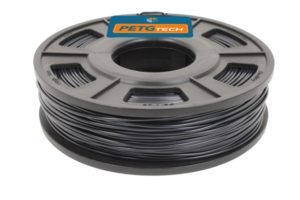
\includegraphics[width=0.5\textwidth,cfbox=azul_marcos 1pt 0pt]{FOTOS/PETG250NEGRO}
\end{figure}
L’adhérence des couches est si ferme que les pièces ont parfois une plus grande résistance à la traction entre les couches que sur l’axe longitudinal de la piste du filament extrudé.
\\\\La résistance entre les couches peut être augmentée en augmentant la température ou en diminuant la vitesse. Cela permet que le matériau fondu soit déposé de manière plus chaude et plus lente. Cependant la finition de la pièce va se détériorer et la transparence sera réduite à cause de la légère déformation des pistes en plastique dû au sur-chauffage.
\\\\Le ventilateur de couche ici intervient en faveur de la transparence du produit et sa finition, mais aussi en faveur de la solidité totale de la pièce.
\\\\Prenez en considération ce qui précède lors de la stratification, en tenant compte du type de la pièce et son utilisation envisagée.
	\subsection{La transparence de PETG}PETG est un matériau translucide comme le PET qui sert à fabriquer des récipients en plastique complètement transparents.
\begin{figure}[H]
\centering
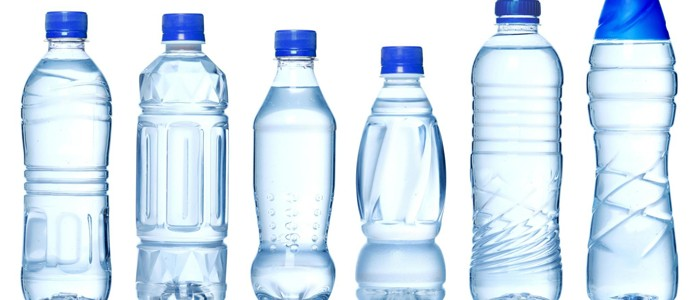
\includegraphics[width=0.5\textwidth,cfbox=azul_marcos 1pt 0pt]{FOTOS/BOTELLASPET}
\end{figure}
Toutefois, Il faut tenir compte du fait que le processus de fabrication de ces récipients diffère tellement de celui utilisé dans l’impression 3D. Et c’est pour cette raison que la réalisation d’une pièce imprimé en 3D entièrement cristalline n'est pas possible, au moins en utilisant la technologie FFF / FDM.
\\\\
Outre l’accumulation des périmètres horizontales, l’augmentation de l’épaisseur des parois des pièces réduit la transparence.
\\\\
Cependant si votre but est d’obtenir des pièces translucides nous vous offrons quelques astuces.
\\\\
En règle générale, plus la température est élevée ou plus la vitesse est basse, alors la transparence de la pièce imprimée serait inférieure. C’est à cause du plastique chaud qui tend à s’écouler, créant des surfaces courbées qui renvoient la lumière.
\\\\
Avec des vitesses plus élevées et des températures plus basses, il est possible de faire en sorte que les pistes en plastique coulées soient déposées de façon plus régulière favorisant la transparence de la pièce.
\\\\
En fonction de l’axe où vous souhaitez avoir une finition plus translucide, vous n’avez qu’à suivre les conseils suivants:
		\subsubsection{La transparence dans l’axe Z (vertical)}La transparence de la pièce va dépendre de la hauteur de la pièce et du remplissage utilisé.
\\\\
Et dépend également du nombre de couches, Alors il est recommandé d’utiliser une plus grande hauteur pour les couches  afin de réduire leurs nombre.
\\\\
Nous devons faire la différence entre les couches qui composent la base de la pièce, et qui sont imprimés directement sur la surface d’impression, et celles qui servent d’enveloppe ou couverture supérieure.
\\\\
Dans les premières couches, la transparence sera bonne car le plastique fondu prend une forme plate et régulière, une fois déposé sur une surface plane.
\\\\
Toutefois les couches supérieures, ont tendance à se courber puisqu’elles reposent sur le périmètre extérieur horizontal pour remplir la structure.
\\\\
C’est pourquoi les couches inférieures ont une meilleure transparence que les couches supérieures.
\\\\
Pour atténuer ce problème, vous pouvez augmenter la vitesse avec laquelle l’imprimante extrude les couches supérieures afin qu’elles soient plus tendues et moins irrégulières.
		\subsubsection{La transparence dans le plan XY (horizontal)}Dans le plan XY la façon pour accroître la transparence c’est de réduire le nombre de périmètres.
\\\\
Cependant si la pièce a une sorte de remplissage, cela va soustraire uniformément la transparence, et on ne peut avoir une transparence élevée qu’avec les pièces faites de verre.
\\\\
Pour ces types de pièces les programmes de stratification offrent l’option d’impression en augmentant la position Z en continu lorsque vous souhaitez imprimer avec un seul périmètre. Cette option est connue par(faire en spiral (Cura), ou le mode de vase (Slic3r et simplifier) et c’est celui que nous recommandons afin d’obtenir les meilleurs résultats en termes de transparence.
\\\\
Comme nous l'avons déjà mentionné, plus la vitesse est élevée et plus la température est basse, plus la transparence est mieux, le résultat dépend d'un arrangement plus régulier et de tendre les pistes en plastique ainsi les essais devraient s’orienter pour trouver la vitesse maximale et la température minimale qui permet d'imprimer Sans séparer les couches.
\\\\
Une vitesse de 70mm/s avec une température de 240\degree et une hauteur de couche de 0,25mm devrait fournir une bonne transparence dans les pièces imprimées en mode vase, bien que cela dépende de la pièce et de la machine.
	\subsection{Le filament PETG 3D et la sécurité alimentaire (FDA Food Safety) des objets 3D imprimés}Le PETG et le PET sont des plastiques très similaires et c’est connu  que ce dernier est largement utilisé dans la fabrication de récipients alimentaires en plastique. C'est parce que les deux ont une certification délivrée par la FDA qui garantit l’hygiène alimentaire entrant en contact avec de tels matériaux.
\begin{figure}[H]
\centering
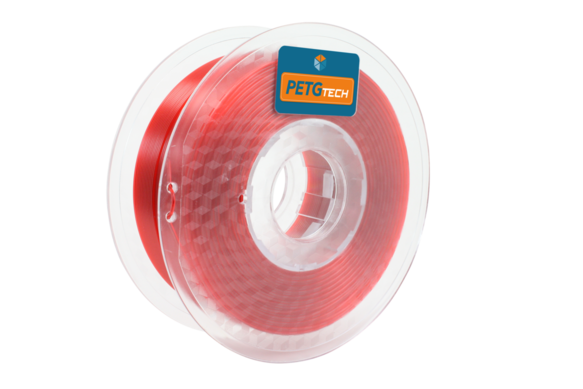
\includegraphics[width=0.5\textwidth,cfbox=azul_marcos 1pt 0pt]{FOTOS/PETGKILOROJO}
\end{figure}
Bien que cela soit vrai, il faut comprendre que la certification fait référence au bouletage (la matière première) à partir de laquelle les filaments de PETG sont produits et que cette certification ne peut être transposée directement pour des raisons différentes que nous allons analyser.
\\\\
Tout d’abord, les filaments d’impression 3D contiennent souvent des additifs afin d’obtenir des caractéristiques qui améliorent leurs performances lorsqu’ils sont utilisés. L’inclusion de tout additif qui n’a pas de certification de la sécurité alimentaire FDA a pour conséquence d’empêcher la validité de la certification.
\\\\
De l’autre côté, la plupart des filaments sont mixtes avec des colorants pour leur donner une couleur, et bien que ces colorants sont certifiés ROHS mais ils ne sont pas certifiés par la sécurité alimentaire FDA.
\\\\
Le premier (ROHS) certifie l’absence d’éléments nocifs (tels que le plomb ou le mercure), tandis que le second certifie la sécurité absolue de l’objet déjà certifié dans la mesure où il serait en contact longtemps avec des aliments destinés à la consommation. De ce fait, la simple addition des colorants non certifiés FDA – empêche ainsi sa validation.
\begin{figure}[H]
\centering
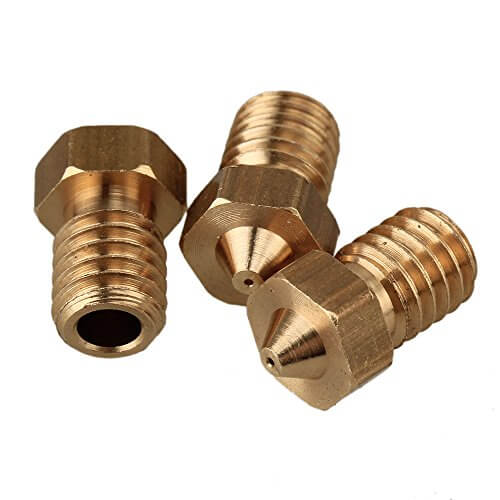
\includegraphics[width=0.5\textwidth,cfbox=azul_marcos 1pt 0pt]{FOTOS/NOZZLES}
\caption*{La buse peut contenir du plomb}
\end{figure}
Même dans le cas de filaments dont matériau de base, les additifs et colorants sont certifiés par la sécurité alimentaire FDA la, le processus d’impression sur un ordinateur à usage domestique le rend non valide à ce certificat.  Il s’agit d’une conséquence des métaux avec laquelle la buse (laiton) et l’extrudeuse qui pousse le filament sont fabriqués.
\\\\
Pour l’ensemble de ce qui précède, il n’est pas possible de créer des objets à l’aide de l’impression 3D de FFF qui sont conformes à la sécurité alimentaire FDA.
\\\\
De ce fait, il est nécessaire d’établir la différence entre la sécurité alimentaire spéciale et générale.
\\\\
La première est accordé par des organismes comme la FDA, qui garantit la sécurité sanitaire et qui sont tenus d’offrir certaines directives de leurs produits.
\\\\
La seconde, la sécurité alimentaire générale, qui fournit l’assurance, selon leurs savoirs et expériences, que quiconque peut avoir tel aliment, et que celui-ci n’est pas nuisible après son utilisation.
\\\\
Quoique les objets imprimés 3D ne puissent pas être certifiés par la FDA, mais il est évident de supposer que personne ne peut devenir intoxiqué en mangeant un cookie qui a été coupé avec un moule de biscuits imprimés en 3D ou à cause d’un verre ou une couverture imprimée 3D.
\begin{figure}[H]
\centering
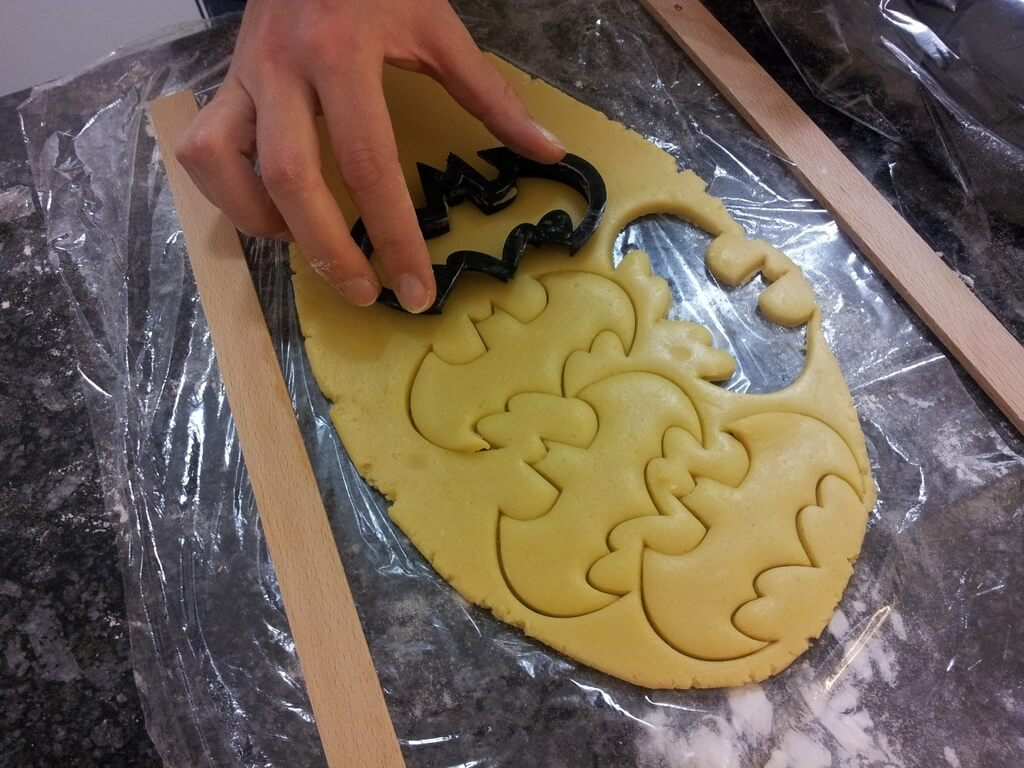
\includegraphics[width=0.5\textwidth,cfbox=azul_marcos 1pt 0pt]{FOTOS/CORTADORGALLETAS}
\end{figure}
Maintenant, il faut tenir compte de certaines choses quand il s’agit de l’impression des objets qui vont être en contact avec des produits alimentaires:
\\\\
L'impression FFF / FDM 3D tend à laisser de petits espaces et interstices sur la surface des pièces ce qui favorisent le développement des bactéries et des microorganismes. Si la pièce est destinée pour une seule utilisation , cela ne cause pas de problème, mais si elle est destinée à être réutilisée alors envisager d’appliquer une  denrées alimentaires pour sceller la surface de la pièce.
\\\\
Ces organismes devraient mourir lors de l’utilisation d’un lave-vaisselle à cause de la température élevée de l’eau, mais cette température peut déformer la pièce.
\\\\
La période de contact entre les aliments et la pièce est importante ; une bouteille n’est pas pareille à une fourchette ou un moule à biscuit.
\section{Problèmes et solutions lors de l’impression 3D avec les filaments PETG}
	\subsection{Problèmes et solutions lors de l’impression 3D avec les filaments PETG}Comment attacher correctement le PETG à la surface d'impression  Le PETG a moins de déformation que l’ABS on peut le contrôler, par contre il est nécessaire que la première couche soit parfaitement collée à la surface d’impression pour avoir une impression satisfaisante.
\\\\
La meilleure méthode à utiliser c’est le lit chaud à 75\degree et à imprimer sur le verre en appliquant une laque standard.
\\\\
Dans le cas où on dispose as de lit chaud, il est recommandé d’utiliser l’option de brim (bord) du programme de stratification et de réduire la vitesse de la première couche de sorte qu’elle soit étroitement collé à la surface d’impression.
\begin{figure}[H]
\centering
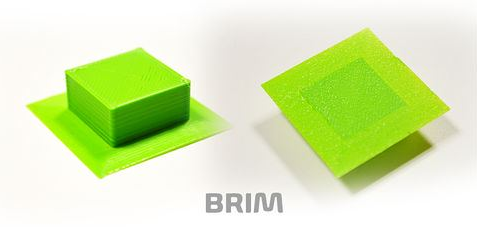
\includegraphics[width=0.5\textwidth,cfbox=azul_marcos 1pt 0pt]{FOTOS/BRIM}
\end{figure}
On a constaté des problèmes lorsque on essaie d’imprimer en 3D avec les filaments PETG sur du ruban bleu (ruban bleu 3M) ou ruban adhésif corporel alors nous vous recommandons d’utiliser la première méthode décrite: laque, verre et lit un à 75\degree.
	\subsection{Les structures de soutien avec le PETG}Nous avons déjà parlé de comment consolider la liaison entre les couches fondu du PETG, mais cela présente un défi  lorsqu’on a affaire avec des pièces qui ont besoin d’une utilisation intensive des supports.
\\\\
Les supports PETG sont retirés avec une telle difficulté que la finition de la surface en contact direct avec ces support est rugueuse et irrégulière.
\\\\
Les programmes de stratification les plus avancées  permettent de configurer la distance horizontale et verticale entre la pièce et les supports, ainsi que le remplissage et la géométrie des structures de soutien.
\\\\
Il est recommandé d’augmenter ces distances, de réduire le remplissage du support et d’opter pour une géométrie simple des lignes au cas où vous rencontrez les problèmes mentionnés ci-dessus, lors de l’utilisation des structures de soutien dans vos pièces.
	\subsection{Problèmes de cordage}La capacité du PETG à se coller fortement le rend susceptible à laisser des débris sous forme de fils dans les pièces imprimées. D’ailleurs, lorsque plusieurs pièces vont être imprimées en même temps, ces petits filets peuvent apparaître entre les pièces puisque la buse doit sauter constamment de l'un à l'autre.
\begin{figure}[H]
\centering
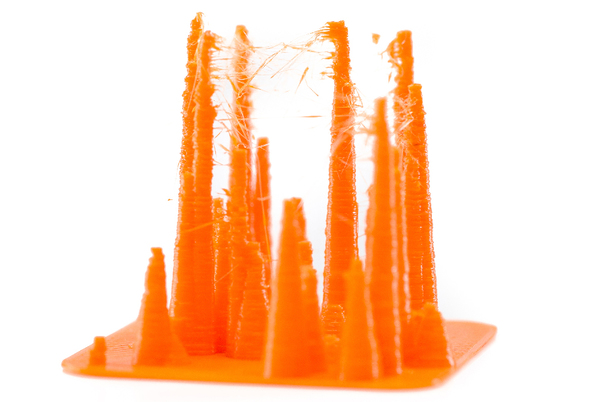
\includegraphics[width=0.5\textwidth,cfbox=azul_marcos 1pt 0pt]{FOTOS/RETRACCION1}
\caption*{Pièces avec problèmes de cordage}
\end{figure}
Comme nous l'avons déjà mentionné, cet effet peut se réduire à l’aide de rétraction, mais il est fortement recommandé que les différentes pièces soient imprimées consécutivement au lieu d’être imprimées simultanément.
\\\\
Nous entendons, par consécutif l’impression complète de la pièce avant de commencer l’impression de la suivante.
\\\\
Ceci est réalisable selon deux manières différentes:
\begin{itemize}
\item L'option triviale est d'imprimer une seule pièce et une fois terminée répéter la même impression autant de fois que voulu.
\item La deuxième alternative, plus avancée et avec certaines limites, consiste à utiliser l'option de stratification que certains programmes proposent, au lieu d'imprimer une pièce à la fois. Vous optez pour La taille maximale des pièces imprimable. en utilisant cette méthode vous dépendrez des dimensions de la buse et la disposition de l'axe de l'imprimante. Nous vous recommandons vivement d'obtenir des informations sur la façon d’utiliser ces options pour ne pas courir le risque d’endommager votre imprimante. Nous vous invitons à vous informer concernant cela à travers les liens suivants:
\end{itemize}
\url{https://www.simplify3d.com/support/tutorials/multi-part-printing/}\\
\url{http://manual.slic3r.org/advanced/sequential-printing}\\
\url{https://ultimaker.com/en/community/3843-force-cura-to-print-objects-separately}
\begin{figure}[H]
  \centering
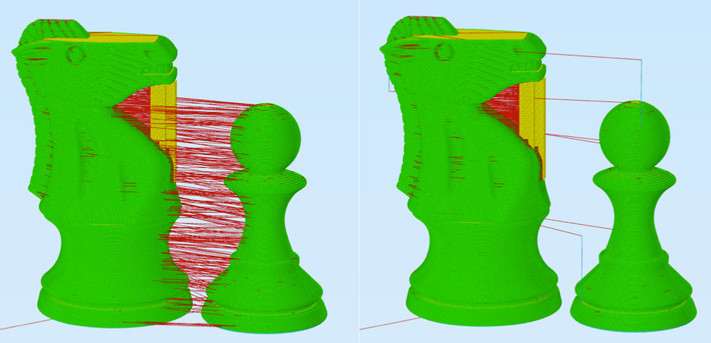
\includegraphics[width=0.5\textwidth,cfbox=azul_marcos 4pt 0pt]{FOTOS/SEQUENTIALPRINTING}
\caption*{Comparaison de l’ acheminement d’impression entre le simultané et le consécutif}
\end{figure}
\section{Souhaitez-vous soutenir notre projet?}
Tous les membres de FFF monde aiment impression 3D et la communauté de la machine. Nous nous estimons chanceux d’être en mesure de travailler sur des projets où nous pouvons vous livrer honnêtement notre passion. À l’avenir, nous aimerions être en mesure de développer plus de matériaux, plus de couleurs et plus de formats. En fin de compte, nous aimerions faire grandir notre entreprise.
\\\\
Par conséquent, une des meilleures actions pour nous aider, si vous le souhaitez et que vous êtes satisfait du filament, est de nous donner 5 étoiles sur Amazon.
\begin{figure}[H]
\centering

\includegraphics[width=0.5\textwidth,cfbox=azul_marcos 1pt 0pt]{FOTOS/AMAZON_FIVE_STARS}
\caption*{Merci beaucoup!}
\end{figure}
\subsection{Autres filaments avec propriétés génial aujourd'hui disponibles dans Amazon}
\begin{description}
  \item[FlexiSMART Tech:] Conçu pour résister à l’abrasion et l’usure des impressions techniques.
\item[ABS Tech:] Effet déformation réduit. Hautes performances sur les applications techniques.
\item[PETG Tech:] Résistance mécanique maximale. Résistance au contact avec l’eau et les rayons UV. Aptitude pour usage alimentaire.
\item[FilaMETAL:] PLA avec une charge métallique non abrasive qui donne une finition mécanique spectaculaire à vos impressions.
\item[PC Tech:] Polycarbonates offrant une résistance élevée à la température et excellentes propriétés mécaniques.
\item[Nylon Tech:] Imprimable à basse température. Résistance aux coups avec un certain degré de flexibilité.
\item[PVA Tech:] Filament soluble dans l’eau destiné pour servir de matériau de support. Excellente compatibilité avec PLA.
\item[HIPS Tech:] Filament soluble dans le Limonène destiné pour servir de matériau de support. Bonne résistance mécanique et excellente compatibilité avec l'ABS.
\end{description}

\includepdf{PDF/FR_CONTRAPORTADA.pdf}
\end{document}
